% !TEX root=../dummy/dummy-05.tex

\chapter{高精度基组外推方法在 CCSD(T) 静态极化率计算上的应用}
\label{sec.5.title}

\section{引言}

静态极化率是光学中问题重要的物理量\cite{Marder-Stucky.ACS.1991};它在化学中,也与 Raman 光谱活性\cite{Wilson-Cross.Dover.1955}、有机反应机理\cite{Xing-Pei.HEP.2005}、以及分子间相互作用\cite{Cohen-Tannoudji-Laloe.Wiley.2020}等问题有概念上的联系。作为计算化学可以导出的物理量,对静态极化率描述的准确与否,也可以用于判断电子结构近似方法精度与有效性。因此,静态极化率是理论与计算化学都十分关心的重要物理量。

相对于静态极化率的概念是动态极化率。动态极化率 $\alpha(\omega)$ 是在特定频率 $\omega$ 的偶极电场扰动下分子能量变化的表征量,而静态极化率是动态极化率在外场频率外推至零的情况即 $\alpha(0)$。本文若不作额外说明,极化率一般指静态极化率。

我们希望对双杂化泛函在静态极化率上的表现作评测与研究;为此,我们需要精确的静态极化率参考值。计算方法的终极目标应当是逼近物理真实的结果,因此参考值应当选取这些真实结果的数值;但现实上,高精度的真实结果难以获得。为了确定参考值以评测近似计算化学方法的有效性,可能的方案是以精确的实验数据、或高精度的计算数据作为参考值。

若要通过实验数据构成参考值以测评理论计算结果,一个关键问题与困难是如何准确地联系理论结果与实验环境\cite{Mata-Suhm.ACIE.2017}。对于静态极化率问题,我们认为,通过实验数据确定与获得参考值较为困难。这种困难不仅来源于实验本身的精度,也同时来源于实验环境的因素本身难于排除;这些因素包括溶剂效应、非谐效应等各种影响,也因静态偶极矩是动态偶极矩在含频电场下频率外推至零的极限、实验上这种外推的矫正难于实现或精确的数据不足。因此,在目前的研究中,电子结构方法的误差经常会被实验本身误差、以及实验环境与理论模拟之间的差距所产生误差的总和所掩盖\cite{Hickey-Rowley.JPCA.2014}。因此,相比起使用实验数值作为参照的方式\cite{Hickey-Rowley.JPCA.2014},大多数对静态极化率的测评工作都使用高精度理论计算数值作为参考值\cite{Hammond-Xantheas.JCP.2009, Huzak-Deleuze.JCP.2013, Wu-Thakkar.CPL.2015, Kozlowska-Bartkowiak.PCCP.2019, Hait-Head-Gordon.PCCP.2018, Beizaei-Sauer.JPCA.2021}。

若要使用理论参考值作测评工作,有两点非常关键。一者,为了确保评测相对来说公平且完整,数据集应当要足够大、且足够多样,以使得测评结果在统计上是有意义的。目前的极化率数据集中,较为接近这一目标的有 Hickey 与 Rowley 设计的 46 分子数据集 (HR46)\cite{Hickey-Rowley.JPCA.2014},Wu、Kalugina 与 Thakkar 设计的 145 分子数据集 (T145)\cite{Wu-Thakkar.CPL.2015}、以及 Hait 与 Head-Gordon 设计的 132 分子与自由基数据集 (HH132)\cite{Hait-Head-Gordon.PCCP.2018}。二者,作为参考值的电子结构理论计算方法应当足够准确。Full-CI/CBS 所给出的结果是最理想的情况,但其计算量巨大,显然是不现实的。HH132 数据集选择使用 CCSD(T)/CBS,即化学中常称为“黄金标准”的 CCSD(T) 方法、并结合有限基组下的 CBS 外推方法\cite{Nyden-Petersson.JCP.1981, Petersson-Mantzaris.JCP.1988},给出了极化率的参考值。其中,对于较小的体系,用于 CBS 外推的模式是 aCV[Q5]Z\footnote{在本文中,我们约定约定,作为双基组 CBS 外推模式,aV[$XY$]Z 代表基组从 aV$X$Z、aV$Y$Z 外推到 aV$\infty$Z 的基组极限近似;aCV[$XY$]Z 代表基组从 aCV$X$Z、aCV$Y$Z 外推到 aV$\infty$Z 的基组极限近似。本工作中,Dunning 系列基组具体的 CBS 外推方式定义于式 (\ref{eq.cbs.zeta3})。本文使用基组简写,同时参考附录 \alertref{sec.A.basis-set};aug-cc-pV$X$Z 将简写为 aV$X$Z,aug-cc-pCV$X$Z 将简写为 aCV$X$Z。};对于较大的体系,用于 CBS 外推的模式是 aCV[TQ]Z\cite{Hait-Head-Gordon.PCCP.2018, Hait-Head-Gordon.JCTC.2018}。这些 CBS 外推所用的基组,几乎已是目前计算化学通常所用的最大基组。对于 CCSD(T) 在电性质计算问题上的准确性,已有文献对此作较为深入的讨论并给出正面的结论\cite{Halkier-Joergensen.JCP.1999, Monten-Deleuze.MP.2011, Hait-Head-Gordon.JCTC.2018}。因此,HH132 数据集的参考值可以认为是可信的。与此同时,HR46 数据集中理论计算给出参考值的模型是 CCSD/aVTZ,而 T145 数据集是 CCSD(T)/aVTZ;CCSD 被认为在计算电性质时精度较低、而 aVTZ 基组也相对较小,因此这两个数据集的理论计算参考值相对于 HH132 数据集,还有进一步提升的空间。

但需要指出,HH132 之所以可以使用 CCSD(T) 结合 aV[TQ]Z 或 aV[Q5]Z 的 CBS 外推模型给出参考值,是因为该数据集最大的分子仅包含 3 个非氢原子 (包括 \ce{BHF2}, \ce{ClCN}, \ce{CO2}, \ce{CSO}, \ce{FCN}, \ce{FCO}, \ce{HCCCl}, \ce{HCCF}, \ce{HCNH2}, \ce{HCOOH}, \ce{NaCN}, \ce{NOCl}, \ce{O3}, \ce{OCl2}, \ce{OF2}, \ce{SCl2}, \ce{SF2}, \ce{SO2})、或 7 个原子 (包括 \ce{CH3NH2});其计算资源需求在较小的体系下是可以接受的。而作为对比,HR46 与 T145 数据集的分子相对来说大许多;HR46 最大的体系包含 15 个原子 (toluene 或 \ce{C7H8});T145 数据集最大的体系包含 14 个原子 (1,4-dithiane 或 \ce{C4H8S2})。HR46 与 T145 数据集中,单个体系含有非氢原子数量最多可达 8 个原子 (例如 6-amino-1\textit{H}-pyrimidin-2-one 或 \ce{C4H5ON3} 以及 5,5,5-trichloropenta-1,3-diyne 或 \ce{C5HCl3})。因此,HR46 与 T145 数据集难以在有限的计算资源下,使用与 HH132 相同的 CCSD(T) 结合大基组 CBS 外推的方式,给出精确的理论计算参考值。

为尽可能地推高 HR46 与 T145 数据集的精度,我们考虑到使用组合化学方法。典型的组合化学方法是 G$n$\cite{Pople-Curtiss.JCP.1989, Curtiss-Pople.JCP.1990, Curtiss-Pople.JCP.1991, Curtiss-Pople.JCP.1998, Curtiss-Raghavachari.JCP.2007} 与 W$n$\cite{Martin-Oliveira.JCP.1999, Parthiban-Martin.JCP.2001};其做法是针对特定的电子结构方法 (如 CCSD(T), CCSD, MP2, HF),使用对应的、代价上可以承受的基组进行计算,并最终合理地依计算层级对这些方法与基组组合的结果作线性的加减处理,给出更为精确的计算结果。FPA 与组合化学方法有着类似的思想\cite{East-Allen.JCP.1993}。由于能量或极化率张量等性质具有可加性,因此可以将总量上占大头的 HF 方法下大基组计算的结果、MP2 与 HF 方法差减部分在中等基组下计算结果、以及计算复杂度最高但总量上较小的 CCSD(T) 与 MP2 方法差减部分在较小基组下的计算结果作加和。这样的结果一般总是比单纯使用低级别的 HF 结合大基组、或高级别的 CCSD(T) 结合小基组要更为准确。FPA 已经应用于计算化学的各种问题,包括反应生成热\cite{East-Allen.JCP.1993, Nielsen-Schaefer.JCP.1997}、构象能\cite{Csaszar-Schaefer.JCP.1998, Tschumper-Tschumper.JCP.2001, Kahn-Kahn.JCC.2008}、非共价相互作用\cite{Tschumper-Quack.JCP.2002, Jurecka-Hobza.PCCP.2006, Marshall-Sherrill.JCP.2011}、激发能\cite{Bokareva-Godunov.IJQC.2008}、核磁共振屏蔽常数\cite{Sun-Xu.JCP.2013, Wang-Xu.JCP.2018}、以及本工作所关心的静态极化率问题\cite{Huzak-Deleuze.JCP.2013, Monten-Deleuze.MP.2011}。

本工作中,我们将着眼于提升 HR46 与 T145 静态极化率数据集的质量至 CCSD(T)/CBS 的精度。为此,我们首先在可以承受 aCV[Q5]Z 级别计算的小分子体系下,对 HF, MP2, CCSD 与 CCSD(T) 作详细的静态极化率基组收敛性分析。这部分工作的目标是确认对于静态极化率问题,FPA 确实可以给出与 HH132 数据集参考值相似精度的结果,即 FPA 是有效的。随后,我们将 FPA 应用于 HR46 与 T145 数据集的参考值计算上;这些参考值的精度将是 CCSD(T)/aCV[Q5]Z 级别的。我们希望这些高精度的参考值能为未来化学工作者在极化率测评,特别是对密度泛函方法的测评上,提供有效的数据来源。

\section{具体方法与实现细节}
\label{sec.5.detail}

\subsection{误差测评标准}

对于一个数据量为 $N$ 的数据集,其参考值是 $\tilde r = \{ r_n \}$;若近似计算方法的结果是 $\tilde c = \{ c_n \}$、以及作为分母的数据 $\tilde d = \{ d_n \}$,那么数据 $\tilde c$ 的相对方均根误差 RelRMSD 定义为
\begin{equation}
    \label{eq.5.relrmsd}
    \text{RelRMSD} (\tilde c, \tilde r, \tilde d) = \sqrt{\frac{1}{N} \sum_{n = 1}^N \left( \frac{c_n - r_n}{d_n} \right)^2} \times 100\%
\end{equation}
不少情况下,参考值 $\tilde r$ 与分母值 $\tilde d$ 是相同的;此情形下将简记 $\text{RelRMSD} (\tilde c, \tilde r, \tilde d)$ 为 $\text{RelRMSD} (\tilde c, \tilde r)$。一般来说,愈低的 RelRMSD 数值,意味着近似计算方法的表现统计上来看愈精确。

RelRMSD 误差多大,才认为是可以被接受或容许的范围?首先,本工作的目标是对较大分子体系的极化率作逼近 CBS 外推模型的 CCSD(T)/aCV[Q5]Z 精度的计算;因此,该级别精度在本工作中视为最精确的参考值 $\tilde r$。由于静态极化率的基组极限误差与实验误差通常在 0.5\% 以内\cite{Brakestad-Frediani.JCTC.2020, Rumble-Rumble.CRC.2021};因此我们认为,对于稍低等级的 FPA 模型或稍小基组下的计算结果,如果其相比于 CCSD(T)/aCV[Q5]Z 的 RelRMSD 误差在 0.5\% 以下,即可认为是足够准确的。

% 关于实验误差,我暂时没能找到 102 版 CRC 常数手册的具体说明。在 2010 年的 90 版 Atomic and Molecular Polarizabilities Table 8 (pdf p. 1648--1649 或 10-200--10-201),注脚中提到了 0.5% 的误差,但也同时指出了实验条件上是含频率的情况、以及数据年代问题。

\subsection{电子结构方法与软件}

本工作的极化率同时使用数值梯度与解析梯度的方式计算。MP2 与 HF 解析极化率是通过 \textsc{PySCF} (commit 3d592b0)的扩展程序脚本 \textsc{dh} (ver 0.1.3) 所实现。正因为该程序可以高效地实现包括双杂化泛函在内的 MP2 型相关能解析极化率,因此本工作中涉及到的所有分子的 MP2 极化率,在引入 RI 近似的前提下,都可以以最精确的 CBS 外推模式 aCV[Q5]Z 实现。对于 CCSD 与 CCSD(T) 方法,本工作使用 \textsc{Q-Chem} (ver 5.1.1)作数值极化率计算。这部分计算将不引入 RI 近似。本工作不对 post-HF 计算过程引入冻核近似。自由基与其他开壳层体系的 HF 自洽场参考态通过自旋非限制性计算给出。

本工作将在 \ref{sec.5.3.1} 小节对极化率的数值与解析之间的误差、RI 近似所导致的误差、以及基组误差进行分析。最终汇报的极化率数值中,HF 与 MP2 是通过 RI 近似下解析给出 (这两个方法将分别记为 RI-JK 与 RI-MP2);CCSD 与 CCSD(T) 的结果将是 RI-MP2 解析极化率、以及更高阶贡献的数值极化率的加和。为更清晰明了地表示极化率数值的构成,本文将使用简记记号;这些记号列于表 \ref{tab.5.1}。该表格的所有记号是针对单个分子或自由基体系的;对于一个数据集合,我们将上标波浪号。举例而言,$\text{RelRMSD} (\symup{\Delta} \tilde \alpha_{\textsf{(2)}/\text{aVTZ}}, \symup{\Delta} \tilde \alpha_{\textsf{(2)}/\text{ref}}, \tilde \alpha_{\textsf{CCSD(T)}/\text{ref}})$ 代表 MP2/aVTZ 同性极化率相对于高精度 MP2 参考值的相对方均根误差;该相对误差计算所用的分母,是高精度 CCSD(T) 参考值。

\begin{table}[t]
\centering
\caption[静态极化率测评的记号定义]{本工作中使用的电子结构方法及其对应极化率的记号\textrm{\textsuperscript{\emph{a}}}。}
\label{tab.5.1}
\widetabular{
    \begin{tabular}{ll}
    \toprule
    记号 & 说明 \\
    \midrule
    num & 数值极化率 \\
    anal & 解析极化率 \\
    conv & 传统电子积分方法,即无 RI 近似的计算方法 \\
    $\alpha$ & 同性极化率 \\
    $\gamma$ & 异性极化率 \\
    $\symup{\Delta} \alpha_\textsf{(2)}$ & $\alpha^\text{anal}_\textsf{RI-MP2} - \alpha^\text{anal}_\textsf{RI-HF}$ \\
    $\symup{\Delta} \alpha_\textsf{D}$ & $\alpha^\text{num}_\textsf{CCSD} - \alpha^\text{num}_\textsf{MP2}$ (不引入 RI 近似) \\
    $\symup{\Delta} \alpha_\textsf{(T)}$ & $\alpha^\text{num}_\textsf{CCSD(T)} - \alpha^\text{num}_\textsf{CCSD}$ (不引入 RI 近似) \\
    $\symup{\Delta} \alpha_\textsf{D(T)}$ & $\alpha^\text{num}_\textsf{CCSD(T)} - \alpha^\text{num}_\textsf{MP2}$ (不引入 RI 近似) \\
    $\symup{\Delta} \alpha_\textsf{HF}$ & $\alpha^\text{anal}_\textsf{RI-HF}$ \\
    $\symup{\Delta} \alpha_\textsf{MP2}$ & $\alpha^\text{anal}_\textsf{RI-MP2} = \alpha_\textsf{HF} + \symup{\Delta} \alpha_\textsf{(2)}$ \\
    $\alpha_\textsf{CCSD}$ & $\alpha^\text{num}_\textsf{CCSD} - \alpha^\text{num}_\textsf{MP2} + \alpha^\text{anal}_\textsf{RI-MP2} = \alpha_\textsf{HF} + \symup{\Delta} \alpha_\textsf{(2)} + \symup{\Delta} \alpha_\textsf{D}$ \\
    $\alpha_\textsf{CCSD(T)}$ & $\alpha^\text{num}_\textsf{CCSD(T)} - \alpha^\text{num}_\textsf{MP2} + \alpha^\text{anal}_\textsf{RI-MP2} = \alpha_\textsf{HF} + \symup{\Delta} \alpha_\textsf{(2)} + \symup{\Delta} \alpha_\textsf{D(T)}$ \\
    \bottomrule
    \end{tabular}
}{
    \item[a] 上述所有应用于同性极化率 $\alpha$ 的记号,将同样应用于异性极化率 $\gamma$。
}
\end{table}

\subsection{数据集}

本工作着重考察的数据集是 HR46 与 T144。原始的 HR46 数据集\cite{Hickey-Rowley.JPCA.2014}包含 46 个体系 (化合物结构参考附录图 \ref{fig.fig-s1});其最精确的计算模型是在 MP2/aVTZ 结构下 CCSD/aVTZ 极化率,且该工作中使用了冻核近似。该数据集的特点是
\begin{itemize}[nosep]
    \item 包含的原子种类较多,包括 H, C, N, O, F, S, P, Cl, Br 等元素;
    \item 在 15 个原子以内的限制下,包含大多数常见有机官能团与无机共价键或离域键;
    \item 分子或自由基的选取契合化学反应、污染控制、生物化学与能源化学的需求;
    \item 除了 3 个体系是自由基体系 (\ce{^2NO}, \ce{^3O2}, \ce{^3SO},上标的数字表示自旋多重度) 为自旋极化体系 (SP),其余体系均为非自旋极化的体系 (NSP)。
\end{itemize}
在本工作中,HR46 中的所有分子的几何结构经过 RI-MP2/aVTZ 级别作优化,且没有启用冻核近似。所有极化率的计算也在此几何结构下实现。

原始的 T145 数据集\cite{Wu-Thakkar.CPL.2015}包含 145 个有机体系。该数据集使用 B3LYP/aVTZ 下的优化结构,最精确的极化率计算模型是 CCSD(T)/aVTZ。T145 数据集是 TABS 数据集\cite{Blair-Thakkar.CTC.2014}的子集。TABS 数据集本身是一大类着眼于药物化学、有机化学与生物化学应用的、自旋非极化的数据集。TABS 数据集的分子数量为 1641;一方面该数据集本身数量较大、另一方面为使该数据集用于机器学习,Blair 等人对 TABS 挑选 298 分子作为极化率与分子容量的训练集,即 T298 数据集\cite{Blair-Thakkar.CPL.2014}。但由于并非所有 T298 数据集中的分子都可以承受 CCSD(T)/aVTZ 的计算代价,因此 Wu 等人从 T298 选出 145 个较小的分子,以给出极化率参考值更精确的数据集,即 T145 数据集\cite{Wu-Thakkar.CPL.2015}。本工作中,我们选取其中的 144 个分子,并称其为 T144 数据集。相比于 T145 数据集,我们排除了第 1363 号分子 (TABS 分子编号,分子名称为 2,3-dihydro-1,3-oxazole);这是因为 TABS 数据集提供的分子构型中,1363 号分子与分子式对应的结构相差两个氢原子,即可能存在数据的损坏。T144 数据集的分子构型使用 TABS 原始数据库提供的 B3LYP/aVTZ 几何结构\cite{Blair-Thakkar.CTC.2014} (化合物结构参考附录图 \ref{fig.fig-s2-1})。

关于 HR46 与 T144 数据集化合物名称的变化与勘定,参考附录 \ref{sec.T145-HR46-name-change}。

本工作的一个关键点是基组收敛性评测。为作有效的评测,测评的体系应可承受高精度大基组 (如 CCSD(T)/aCV5Z 级别模型) 的计算量与资源需求。在 HR46 与 T144 数据集中,14 个体系 (\ce{Cl2}, \ce{CO}, \ce{CO2}, \ce{H2O}, \ce{N2}, \ce{NH3}, \ce{^3O2}, \ce{PH3}, \ce{SH2}, \ce{SiH4}, \ce{^3SO}, \ce{SO2}, \ce{FCN}, \ce{HCHS}) 可以承受大计算量的计算。这 14 个数据也同样出现在 HH132 数据集中。在测评基组收敛性问题时,这 14 个小体系的分子构型将采用 NIST 计算化学数据库中实验的数据\cite{NIST.CCCBDB};这些构型也同样为 HH132 数据集所采用。

\subsection{基组与 RI 近似}

在本工作中,我们将使用 Dunning 系列基组 aV$X$Z 与 aCV$X$Z。H 与 Br 原子并不出现在 aCV$X$Z 系列基组中;对于这两个原子作 aCV$X$Z 级别计算时,将不加说明地替换为对应的 aV$X$Z 基组。RI 近似可以大幅减少 MP2 的计算耗时,并且不会产生严重的误差损耗,是性价比相当高的技术手段\cite{Vahtras-Feyereisen.CPL.1993}。本工作的解析极化率计算中,我们对 Weigend 算法实现的 RI-JK\cite{Weigend-Weigend.PCCP.2002} 与 RI-MP2 相关贡献\cite{Weigend-Haettig.JCP.2002}计算均使用 ETB 自动辅助基;等比参数设为 \textsc{PySCF} 程序默认的 $\beta = 2$。由于基于 \textsc{PySCF} 的扩展程序 \textsc{dh} 的高效率实现、以及对大基组下内存的合理控制,使得本工作中所有体系都可以在 MP2/aCV5Z 下完成计算。作为自洽场的 RI-JK 方法的能量收敛精度为 $10^{-10}$ Hartree。

\subsection{数值极化率}

在附录 \alertref{sec.3.title} 中,我们已经了解极化率是对外电场强度的二阶梯度;依外电场 $\pmb{\mathcal{E}}$ 在三个空间方向取向的大小 $(\mathcal{E}_x, \mathcal{E}_y, \mathcal{E}_z)$,极化率张量 $\bm{\alpha}$ 是 $3 \times 3$ 的对称矩阵:
\begin{equation}
    \alpha_{ts} = - \frac{\partial^2 E}{\partial \mathcal{E}_t \partial \mathcal{E}_s} \quad t, s \in \{ x, y, z \}
\end{equation}
作为物理上可观测的量,本工作着重测评同性极化率 $\alpha$\footnote{通过非加粗的标量记号表示,用以区分作为矩阵的极化率张量 $\bm{\alpha}$。}和异性极化率 $\gamma$:
\begin{align}
    \alpha &= \frac{1}{3} \left( \alpha_{xx} + \alpha_{yy} + \alpha_{zz} \right) = \mathrm{tr} (\bm{\alpha}) \\
    \gamma &= \frac{1}{\sqrt{2}} \left( (\alpha_{xx} - \alpha_{yy})^2 + (\alpha_{yy} - \alpha_{zz})^2 + (\alpha_{zz} - \alpha_{xx})^2 + 6 (\alpha_{xy}^2 + \alpha_{yz}^2 + \alpha_{zx}^2) \right)^{1/2}
\end{align}
对于数值极化率的求取过程,对角元部分 $\alpha_{tt}$ ($t \in \{ x, y, z \}$) 通过线性的三点格式作数值导数给出:
\begin{equation}
    \label{eq.pol-findiff-alpha-def}
    \alpha_{tt} = - \frac{\partial^2 E}{\partial \mathcal{E}_t^2} = - \frac{1}{h^2} \left( E(- \bm{h}_t) - 2 E(\bm{0}) + E(\bm{h}_t) \right) + o(h^2)
\end{equation}
非对角元部分 $\alpha_{ts}$ ($t, s \in \{ x, y, z \}, \, t \neq s$) 通过平面上的三点格式作数值导数给出:
\begin{align}
    \label{eq.pol-findiff-gamma-def}
    \alpha_{ts} &= - \frac{\partial^2 E}{\partial \mathcal{E}_t \partial \mathcal{E}_s} \notag\\
    &= - \frac{1}{4h^2} \left( E(- \bm{h}_t - \bm{h}_s) - E(- \bm{h}_t + \bm{h}_s) - E(\bm{h}_t - \bm{h}_s) + E(\bm{h}_t + \bm{h}_s) \right) + o(h^2)
\end{align}
其中,$\bm{h}_t, \bm{h}_s$ 分别是 $t, s$ 方向外加微扰电场强度矢量:
\begin{equation*}
    \bm{h}_x = (h, 0, 0)^\dagger, \quad \bm{h}_y = (0, h, 0)^\dagger, \quad \bm{h}_z = (0, 0, h)^\dagger
\end{equation*}
标量 $h$ 是微扰电场的强度;在本工作的数值差分计算中,我们对所有体系均使用 $h = 0.004$ au。关于使用该外加微扰强度的合理性,我们在附录的 \ref{sec.5.s9} 小节中作讨论。

数值梯度计算大多使用 \textsc{Q-Chem}。自洽场收敛判据 (\texttt{SCF\_CONVERGENCE} 关键词) 设为 $10^{-11}$ au,CCSD 能量与振幅收敛判据 (\texttt{CC\_E\_CONV} 与 \texttt{CC\_T\_CONV}) 分别设为 $10^{-10}$ au 与 $10^{-7}$ au。作为特例,对于 \ce{^2NO} 分子,其数值梯度是通过 \textsc{PySCF} 在限制分子对称性的不可约表示而实现;其自洽场与 CCSD 收敛判据与 \textsc{Q-Chem} 设置相同。由于我们在以 aCV5Z 基组计算 \ce{SO2} 分子时遇到收敛困难,因此该情形下我们分别降低 \textsc{Q-Chem} 的收敛判据 \texttt{SCF\_CONVERGENCE}, \texttt{CC\_E\_CONV}, \texttt{CC\_T\_CONV} 为 $10^{-10}$ au, $10^{-9}$ au, $10^{-6}$ au。

\subsection{CBS 外推}
\label{sec.5.cbs}

CBS 外推方法通常被认为在计算资源不足、以及有限基组不充分大时,可以有效地提升计算精度以更接近完备基组极限的手段。关于具体的 CBS 外推方法与策略,目前已有许多文献对此作说明与讨论\cite{Nyden-Petersson.JCP.1981, Petersson-Mantzaris.JCP.1988, Dunning-Dunning.JCP.1989, Peterson-Dunning.JCP.1994, Jensen-Jensen.TCA.2005, Karton-Martin.TCA.2006, Truhlar-Truhlar.CPL.1998, Klopper-Kutzelnigg.JMST.1986, Kutzelnigg-Morgan.JCP.1992, Martin-Martin.CPL.1996, Helgaker-Noga.JCP.1997, Halkier-Wilson.CPL.1998, Halkier-Olsen.CPL.1999}。HH132 数据集的原始工作使用的 CBS 策略是三次外推式\cite{Hait-Head-Gordon.PCCP.2018}
\begin{equation}
    \label{eq.cbs.zeta3}
    \alpha(\zeta) = \alpha(\text{CBS}) + A \zeta^{-3}
\end{equation}
其中,$\zeta$ 是基组的基数。对于 Dunning 基组,aV$X$Z 或 aCV$X$Z 的 $X = \mathrm{D, T, Q, 5}$ 分别对应的基数是 $\zeta = 2, 3, 4, 5$。对于 CBS 外推模型 aCV[TQ]Z,其相对于 aCV5Z 的误差,对于偶极矩大约是 $\sim 0.2\%$\cite{Hait-Head-Gordon.JCTC.2018, Halkier-Joergensen.JCP.1999},对于极化率大约是 $\sim 0.1\%$\cite{Hait-Head-Gordon.PCCP.2018};这意味着三次外推式 (\ref{eq.cbs.zeta3}) 对电性质的计算是有效的。在本工作中,对极化率的计算将沿用该 CBS 外推策略。对于 HR46 与 T144 全部分子的 MP2 极化率的计算,我们都使用 aCV[Q5]Z 作为参考值;而对于 CCSD 与 CCSD(T) 计算,则会依照分子体系的大小而给予相适应的 CBS 外推模型 aV[$XY$]Z ($[XY] = \mathrm{[Q5], [TQ], [DT]}$) 计算。

\subsection{FPA 策略}

在有限的计算资源内,若高等级方法难以直接计算得到,那么 FPA 方法会是一种尽可能逼近高等级计算方法结果、但使用相对较小计算资源的手段。在本工作中,我们的目标是给出 CCSD(T)/CBS 的参考值,其中的 CBS 是通过高精度的 aCV[Q5]Z 外推近似得到。考虑到不是所有体系都可以承受如此大的计算量,因此对极化率作三部分拆分:以同性极化率为例,CCSD(T) 极化率 $\alpha_\textsf{CCSD(T)}$ 拆分出这三部分是 HF 部分 $\alpha_\textsf{HF}$、MP2 相关贡献部分 $\symup{\Delta} \alpha_\textsf{(2)}$、以及更高阶贡献部分 $\symup{\Delta} \alpha_\textsf{D(T)}$:
\begin{align}
    \alpha_{\textsf{CCSD(T)}/\text{CBS}} &= \alpha_{\textsf{HF}/\text{CBS}} + \symup{\Delta} \alpha_{\textsf{(2)}/\text{CBS}} + \symup{\Delta} \alpha_{\textsf{D(T)}/\text{CBS}} \notag\\
    &\simeq \alpha_{\textsf{HF}/\text{LB}} + \symup{\Delta} \alpha_{\textsf{(2)}/\text{CBS}} + \symup{\Delta} \alpha_{\textsf{D(T)}/\text{CBS}'} \notag\\
    &\simeq \alpha_{\textsf{HF}/\text{LB}} + \symup{\Delta} \alpha_{\textsf{(2)}/\text{CBS}} + \symup{\Delta} \alpha_{\textsf{D(T)}/\text{SB}}
\end{align}
上式下标的 LB 是指大基组 (large basis set)、SB 是指小基组 (small basis set)。我们的工作对 HF 方法直接采用 $\text{LB} = \text{aCV5Z}$ 基组。对于 MP2 的相关贡献部分 $\symup{\Delta} \alpha_{\textsf{(2)}/\text{CBS}}$,我们始终选择使用最高精度的 aCV[Q5]Z 外推模型。更高阶贡献部分 $\symup{\Delta} \alpha_{\textsf{D(T)}/\text{CBS}'}$ 是指对高精度 CBS 外推 $\symup{\Delta} \alpha_{\textsf{D(T)}/\text{CBS}}$ 的近似;目前针对 $\symup{\Delta} \alpha_{\textsf{D(T)}/\text{CBS}'}$ 的计算基组级别取决于体系的大小。若对 $\symup{\Delta} \alpha_{\textsf{D(T)}/\text{CBS}'}$ 的计算使用基组 aV[$XY$]Z 与 aCV[$XY$]Z,那么我们称该 FPA 策略为 FPA-aV[$XY$]Z 与 FPA-aCV[$XY$]Z。同样地,若对 $\symup{\Delta} \alpha_{\textsf{D(T)}/\text{SB}}$ 的计算使用基组 aV$X$Z 与 aCV$X$Z ($X < 5$),那么我们称该 FPA 策略为 FPA-aV$X$Z 与 FPA-aCV$X$Z。

\begin{figure}[ht]
    \centering
    \caption[静态极化率计算的 FPA 模型]{本工作所使用的 FPA 模型。该图以 FPA-aV[TQ]Z 作为例子;其中 $\alpha_{\textsf{HF}/\text{LB}}$ 以 aCV5Z 计算所得、$\symup{\Delta} \alpha_{\textsf{(2)}/\text{CBS}}$ 以 aCV[Q5]Z 计算所得、$\symup{\Delta} \alpha_{\textsf{D(T)}/\text{CBS}'}$ 以 aV[TQ]Z 计算所得。}
    \label{fig.fig-1}
    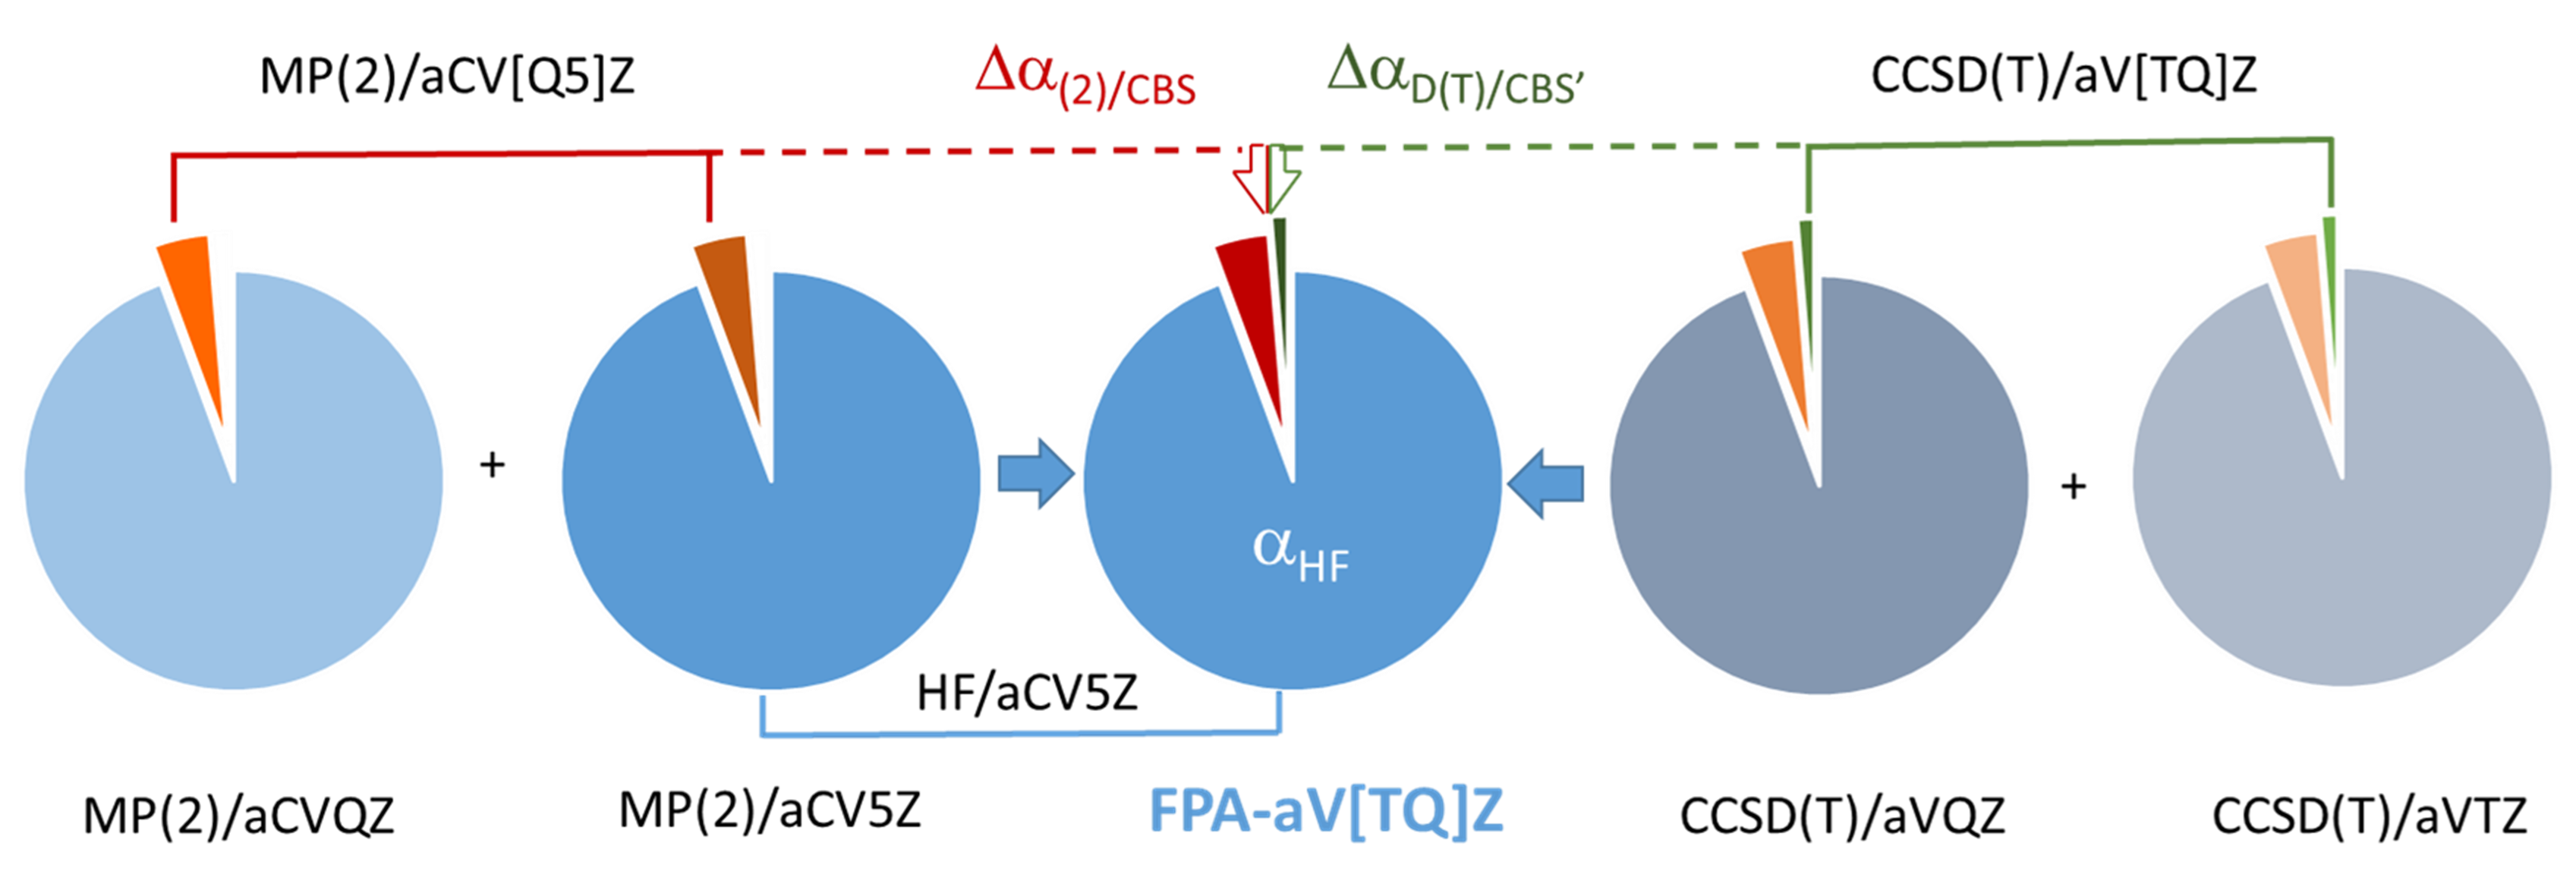
\includegraphics[width=0.9\textwidth]{assets/fig-1.png}
\end{figure}

以 FPA-aV[TQ]Z 作为例子,使用 FPA 策略的合理性通过图 \ref{fig.fig-1} 展示。HF 方法的结果占真实结果的绝对大头;但为正确描述物性,高质量的相关效应描述也是重要的。由于 HF 方法一般来说依基组基数 $\zeta$ 的收敛速度相当快\cite{Jensen-Jensen.TCA.2005, Karton-Martin.TCA.2006},因此许多 CBS 策略、包括 HH132 数据集的参考值,都对 HF 方法直接使用计算量上最大可承受的基组。而对于相关效应,则依基组基数 $\zeta$ 的增大,收敛速度相对缓慢。大多数情况下,MP2 占据相关效应的主要部分;因此,对 MP2 的大基组精确描述也非常重要。但对于更高阶的相关效应,一方面其绝对数值已然较小,另一方面数值对基组基数 $\zeta$ 的敏感性较小、或相对于 MP2 相关效应的收敛速度更快。对于后一方面所述的现象,目前已经在核磁屏蔽常数的计算\cite{Sun-Xu.JCP.2013, Wang-Xu.JCP.2018, Gregusova-Bartlett.JCTC.2010}、能量计算\cite{Truhlar-Truhlar.CPL.1998}等诸多情形下有所验证。因此,我们也会期望在极化率问题中,对于 CCSD(T) 相对于 MP2 之间的高级相关效应,使用较低等级基组或 CBS 外推方法,也可以提供一个合理的对高等级 CBS 外推方法的近似。本工作的其中一个重点,即是验证这个猜想的合理性。

\section{结论与讨论}

\subsection{RI 误差与数值差分误差}
\label{sec.5.3.1}

在本工作中,HF 与 MP2 的极化率是通过解析梯度给出,但引入了 RI 近似;CCSD 与 CCSD(T) 尽管未使用 RI 近似,但引入了数值差分误差。注意到表 \ref{tab.5.1} 中,将要汇报的 $\alpha_\textsf{CCSD(T)}$ 参考值是由 $\alpha^\text{anal}_\textsf{RI-MP2} + \symup{\Delta} \alpha^\text{num}_\textsf{D(T)}$ 两部分构成;这两部分分别包含 RI 近似误差与数值差分误差。为了估计这部分误差的大小,我们考察了 HF 与 MP2 方法在 aVTZ 基组下、包含 RI 近似与不使用 RI 近似的同性极化率结果。

我们看到,解析 RI-HF 与数值 HF 方法同性极化率之间相对方均根误差 $\text{RelRMSD} (\tilde \alpha_\textsf{RI-HF}^\text{anal}, \tilde \alpha^\text{num}_\textsf{HF})$,对于 HR46 与 T144 数据集,分别是 0.018\% 与 0.022\%。解析 RI-MP2 与数值 MP2 方法相关能贡献部分的方均根误差 $\text{RelRMSD} (\symup{\Delta} \tilde \alpha^\text{anal}_\textsf{RI-(2)}, \allowbreak \symup{\Delta} \tilde \alpha^\text{num}_\textsf{(2)}, \allowbreak \tilde \alpha^\text{num}_\textsf{MP2})$,对于两个数据集的误差均小于 0.01\%。这些误差都远远小于实验误差标准的 0.5\%,因此我们认为 RI 近似与数值差分误差对总的同性极化率 $\alpha_\textsf{CCSD(T)}$ 计算结果影响相当小,以至于可以忽略。我们猜测该结论对异性极化率 $\gamma_\textsf{CCSD(T)}$ 也同样适用。

我们还看到,对于相关贡献部分,自洽场收敛条件会对数值差分误差有一定影响。相关的数据与结论列于附录的 \ref{sec.5.s9} 小节。

\subsection{小体系的同性极化率基组收敛性}

在这两小节中,我们将对 14 个小体系 (\ce{Cl2}, \ce{CO}, \ce{CO2}, \ce{H2O}, \ce{N2}, \ce{NH3}, \ce{^3O2}, \ce{PH3}, \ce{SH2}, \ce{SiH4}, \ce{^3SO}, \ce{SO2}, \ce{FCN}, \ce{HCHS}) 作系统的基组收敛性分析,并籍此确定用于计算同性极化率的、高效同时精确的 FPA 模型。在该分析中,参考值由 CCSD(T)/CBS 计算所得:
\begin{equation}
    \alpha_{\textsf{CCSD(T)}/\text{CBS}} = \alpha_{\textsf{HF}/\text{aCV5Z}} + \symup{\Delta} \alpha_{\textsf{(2)}/\text{aCV[Q5]Z}} + \symup{\Delta} \alpha_{\textsf{D(T)}/\text{aCV[Q5]Z}}
\end{equation}
该参考值也对应了 HH132 数据集中最精确的 CBS 外推模型。详细的对 Dunning 系列基组的误差分析展示于表 \ref{tab.5.2}。

\begin{table}[!t]
\centering
\caption[14 个小体系同性极化率 RelRMSD]{14 个小体系同性极化率的相对方均根误差\textrm{\textsuperscript{\emph{a}}}。}
\label{tab.5.2}
\widetabular{
    \begin{tabular}{cld{2.4}d{2.4}d{2.4}d{2.4}}
    \toprule
          &              & \multicolumn{4}{c}{RelRMSD / \%}                \\ \cmidrule(lr){3-6}
    基组基数 & \multicolumn{1}{c}{基组}    &
      \multicolumn{1}{c}{$\tilde \alpha_\textsf{HF}$\tnote{b}}  &
      \multicolumn{1}{c}{$\symup{\Delta} \tilde \alpha_\textsf{(2)}$\tnote{c}}  &
      \multicolumn{1}{c}{$\symup{\Delta} \tilde \alpha_\textsf{D}$\tnote{c}} &
      \multicolumn{1}{c}{$\symup{\Delta} \tilde \alpha_\textsf{D(T)}$\tnote{c}}     \\ \midrule
    2-$\zeta$ & aVDZ         & 3.385       & 0.853       & 1.113      & 0.787          \\
              & aCVDZ        & 3.376       & 0.799       & 1.053      & 0.748          \\ \midrule
    3-$\zeta$ & aVTZ         & 0.703       & 0.516       & 0.406      & 0.297          \\
              & aCVTZ        & 0.671       & 0.385       & 0.339      & 0.270          \\
              & aV[DT]Z      &             & 0.535       & 0.155      & \textbf{0}.\textbf{144} \\
              & aCV[DT]Z     &             & 0.373       & 0.156\tnote{d}     & 0.178\tnote{d}         \\ \midrule
    4-$\zeta$ & aVQZ         & 0.097       & 0.403       & 0.168      & 0.124          \\
              & aCVQZ        & 0.084       & 0.244       & 0.120      & 0.101          \\
              & aV[TQ]Z      &             & 0.359       & 0.111      & \textbf{0}.\textbf{086} \\
              & aCV[TQ]Z     &             & 0.179       & 0.131\tnote{e}     & 0.096\tnote{e}         \\ \midrule
    5-$\zeta$ & aV5Z         & 0.024       & 0.233       & 0.082      & 0.065          \\
              & aCV5Z        & \multicolumn{1}{c}{\textbf{0}\tnote{f}} & 0.125       & 0.061      & 0.052          \\
              & aV[Q5]Z      &             & 0.071       & 0.013      & \textbf{0}.\textbf{017} \\
              & aCV[Q5]Z     &             & \multicolumn{1}{c}{\textbf{0}\tnote{f}} & \multicolumn{1}{c}{0\tnote{f}}         & \multicolumn{1}{c}{0\tnote{f}}             \\
    \bottomrule
    \end{tabular}
}{
    \item[a] 粗体的数字表示除参考值模型 FPA-aCV[Q5]Z 外,不同计算水平下最佳的 FPA 模型;即依 3,4,5-$\zeta$ 分类下 FPA-aV[DT]Z、FPA-aV[TQ]Z 与 FPA-aV[Q5]Z。
    \item[b] HF 同性极化率相对方均根误差为 $\text{RelRMSD} (\tilde \alpha_{\textsf{HF}/\text{basis}}, \tilde \alpha_{\textsf{HF}/\text{ref}}, \tilde \alpha_{\textsf{CCSD(T)}/\text{ref}})$。其中,$\tilde \alpha_{\textsf{HF}/\text{ref}}$ 指代的是 $\tilde \alpha_{\textsf{HF}/\text{aCV5Z}}$,$\tilde \alpha_{\textsf{CCSD(T)}/\text{ref}}$ 指代的是作为参考值的 $\alpha_{\textsf{CCSD(T)}/\text{CBS}}$。
    \item[c] 相关能贡献的同性极化率相对方均根误差为 $\text{RelRMSD} (\symup{\Delta} \tilde \alpha_{\textsf{corr}/\text{basis}}, \symup{\Delta} \tilde \alpha_{\textsf{corr}/\text{ref}}, \tilde \alpha_{\textsf{CCSD(T)}/\text{ref}})$。其中,$\symup{\Delta} \tilde \alpha_{\textsf{corr}}$ 可以是指 $\symup{\Delta} \tilde \alpha_{\textsf{(2)}}$、$\symup{\Delta} \tilde \alpha_{\textsf{D}}$ 或 $\symup{\Delta} \tilde \alpha_{\textsf{D(T)}}$;而 $\symup{\Delta} \tilde \alpha_{\textsf{corr}/\text{ref}}$ 指代的是 $\symup{\Delta} \tilde \alpha_{\textsf{corr}/\text{aCV[Q5]Z}}$。
    \item[d] 在排除 \ce{^3O2} 与 \ce{^3SO} 体系后,$\symup{\Delta} \tilde \alpha_\textsf{D}$ 与 $\symup{\Delta} \tilde \alpha_\textsf{D(T)}$ 的 RelRMSD 误差分别降至 0.126\% 与 0.136\%。对于这两个体系的基组收敛分析,将在附录 \ref{sec.5.s4} 小节展开。
    \item[e] 在排除 \ce{Cl2} 体系后,$\symup{\Delta} \tilde \alpha_\textsf{D}$ 与 $\symup{\Delta} \tilde \alpha_\textsf{D(T)}$ 的 RelRMSD 误差分别降至 0.089\% 与 0.069\%。对于该体系的基组收敛分析,将在附录 \ref{sec.5.s4} 小节展开。
    \item[f] 这些数值依据参考值的选取方式,从定义上是零。
}
\end{table}

首先,从具体的计算结果来看,首先可以肯定的是 HF 方法所给出的同性极化率确实占总同性极化率的主要部分;而 MP2 相关效应所贡献的部分,一般来说要比更高阶相关效应的部分要大一些。总的相关效应对于同性极化率上可能是正也可能是负;MP2 贡献部分与更高阶贡献部分的正负号经常是相反的。因此,为给出非常精确的极化率数据,我们需要仔细地分别考虑每个贡献部分的数值。

从表 \ref{tab.5.2} 总结的数据来看,我们发现对于 HF 方法而言,$\tilde \alpha_\textsf{HF}$ 的相对方均根误差在 2-$\zeta$ 基组下的误差相当大 ($> 3\%$)。因此,在极化率计算中,即使引入了弥散基组,2-$\zeta$ 级别下的计算结果也不具有实用性。在 3-$\zeta$ 基组下,$\tilde \alpha_\textsf{HF}$ 的相对方均根误差骤降至 0.7\%;到 4-$\zeta$ 基组时已经降至 0.1\% 以下,依基组基数 $\zeta$ 的收敛速度非常快。因此,我们可以放心地认为在 aCV5Z 基组下,HF 方法的同性极化率已经非常精确、而不需要特意作额外 CBS 外推。该分析也印证了 HH132 数据集参考值构建过程中对 HF 方法的处理方式是合理的\cite{Hait-Head-Gordon.PCCP.2018}。

一个有意思的现象是,$\tilde \alpha_\textsf{HF}$ 的相对方均根误差在 2-$\zeta$ 与 3-$\zeta$ 等小基组下误差比对应的相关部分贡献 $\symup{\Delta} \tilde \alpha_\textsf{corr}$ 更大;但当基组到 4-$\zeta$ 时,相关效应的误差比 HF 反过来更大。注意到 4-$\zeta$ 时,$\tilde \alpha_\textsf{HF}$ 的相对方均根误差是 0.1\% 以下;但对于 $\symup{\Delta} \tilde \alpha_\textsf{(2)}$ 则在 aCVQZ 下是 0.244\%、aVQZ 下是 0.403\%。这些误差表现可以说明,MP2 相关效应贡献的部分依基组基数 $\zeta$ 的收敛速度相对于 HF 而言慢得多;这也与 HH132 的测评结论一致\cite{Hait-Head-Gordon.PCCP.2018}。同时,我们看到,若在 4-$\zeta$ 与 5-$\zeta$ 级别的基组上引入 CBS 外推,则误差可以降低大约 0.05\%;并且当引入核层基函数时,极化率的误差表现普遍更低一些。考虑到即使是 4-$\zeta$ 的 CBS 下 $\symup{\Delta} \tilde \alpha_\textsf{(2)}$ 仍有一定的误差、且在引入了 RI 近似后 MP2 的计算量在更大的 5-$\zeta$ 下是可接受的;那么为了与 HH132 的参考值维持尽可能相似的精度,我们采用 aCV[Q5]Z 的 CBS 外推模型计算 $\symup{\Delta} \alpha_\textsf{(2)}$ 的参考值。至此,同性极化率在精度上可以提升的空间,就是如何精确且高效地计算 $\symup{\Delta} \alpha_\textsf{D(T)}$ 的结果。

幸运的是,从表 \ref{tab.5.2} 的数据来看,$\symup{\Delta} \tilde \alpha_\textsf{D(T)}$ 的相对方均根误差,比起 $\symup{\Delta} \tilde \alpha_\textsf{(2)}$ 来说依基组基数 $\zeta$ 的收敛速度更快且误差更小。举例而言,对于 aVTZ 与 aVQZ 基组,$\symup{\Delta} \tilde \alpha_\textsf{D(T)}$ 相对方均根误差为 0.297\% 与 0.124\%,在数值上与收敛速度上都明显快于 $\symup{\Delta} \tilde \alpha_\textsf{(2)}$ 的 0.516\% 与 0.403\%。对于 aVTZ 与 aVQZ 基组,引入 CBS 外推得到 aV[DT]Z 与 aV[TQ]Z 后,其误差可以有大约一半的降幅,且两个 CBS 外推模型的误差都小于 0.2\%。同时,aV[Q5]Z 外推模型相比于 aCV[Q5]Z 的误差是非常小的 0.017\%。

需要指出,对于如 $\symup{\Delta} \alpha_\textsf{D(T)}$ 高阶的相关贡献部分,基组中引入核层的函数不仅会大幅增加计算消耗,同时对部分体系也会破坏收敛趋势、以至于 CBS 外推模型失效。举例而言,对于我们目前研究的 14 个小体系,$\symup{\Delta} \tilde \alpha_\textsf{D(T)}$ 在 aCV[DT]Z 外推下的相对方均根误差是 0.178\%,比 aV[DT]Z 的 0.144\% 要更大;只有当排除了 \ce{^3O2} 与 \ce{^3SO} 这两个异常体系,误差才能降至比 aV[DT]Z 更低的 0.136\%。类似的情形在 aCV[TQ]Z 与 aV[TQ]Z 的比较中也存在。对于这些异常体系的讨论,我们在附录 \ref{sec.5.s4} 小节中展开。

综上所述,我们建议对同性极化率使用的 FPA 模型是
\begin{equation}
    \label{eq.5.fpa-alpha}
    \alpha_{\text{FPA-aV[}XY\text{]Z}} = \alpha_{\textsf{HF}/\text{aCV5Z}} + \symup{\Delta} \alpha_{\textsf{(2)}/\text{aCV[Q5]Z}} + \symup{\Delta} \alpha_{\textsf{D(T)}/\text{aV[}XY\text{]Z}}
\end{equation}
其中,$[XY]$ 依据分子大小可以取为 $\mathrm{[DT], [TQ], [Q5]}$。相对于最佳的理论计算模型 $\alpha_{\text{FPA-aCV[Q5]Z}}$,$\alpha_{\text{FPA-aV[}XY\text{]Z}}$ 的误差来源仅出现在 $\symup{\Delta} \tilde \alpha_\textsf{D(T)}$ 的基组不完备程度。因此,从表 \ref{tab.5.2} 的数据来看,FPA-aV[DT]Z、FPA-aV[TQ]Z、FPA-aV[Q5]Z 在计算同性极化率时的相对方均根误差分别是 0.144\%、0.086\%、0.017\%。这些 FPA 模型的误差都明显小于我们的目标精度 0.5\%。我们期待这些 FPA 模型应用于更大体系、如 HR46 或 T144 中更大的分子时,计算精度可以与 HH132 的参考值相比较。

\subsection{自旋非极化小体系的异性极化率基组收敛性}

本工作同样考虑了异性极化率 $\gamma$ 的计算问题。在这一小节中,我们考虑 7 个自旋非极化分子 (\ce{Cl2}, \ce{CO}, \ce{CO2}, \ce{FCN}, \ce{HCHS}, \ce{N2}, \ce{SO2}) 的基组收敛性与 CBS 外推精度,以确定对异性极化率计算所适合使用的 FPA 模型。相对于同性极化率分析过程中使用的 14 个体系,我们排除了 5 个自旋非极化与 2 个自旋极化分子。其中,5 个自旋非极化分子 (\ce{H2O}, \ce{H2S}, \ce{NH3}, \ce{PH3}, \ce{SiH4}) 由于异性极化率的数值过小 (小于 0.5 $\text{\AA}{}^3$),使用相对方均根误差对这些分子作分析不是非常合理。在附录的表 \ref{tab.5.s7} 中,我们使用绝对值的方均根误差作为判标,将这 5 个小分子引入基组收敛性与 CBS 外推精度分析,并且认为引入这 5 个异性极化率 $\gamma$ 较小的体系不影响结论。同时,由于 HR46 与 T144 的绝大多数分子都是自旋非极化分子;在对异性极化率的讨论中,我们将局限于自旋非极化体系,因此排除了自旋极化体系 \ce{^3O2} 与 \ce{^3SO}。详细的对 Dunning 系列基组的误差分析展示于表 \ref{tab.5.3}。

\begin{table}[!ht]
\centering
\caption[7 个自旋非极化小体系异性极化率 RelRMSD]{7 个自旋非极化小体系异性极化率的相对方均根误差\textrm{\textsuperscript{\emph{a}}}。}
\label{tab.5.3}
\widetabular{
    \begin{tabular}{cld{2.4}d{2.4}d{2.4}d{2.4}}
    \toprule
          &              & \multicolumn{4}{c}{RelRMSD / \%}                \\ \cmidrule(lr){3-6}
    基组基数 & \multicolumn{1}{c}{基组}    &
      \multicolumn{1}{c}{$\tilde \gamma_\textsf{HF}$\tnote{b}}  &
      \multicolumn{1}{c}{$\symup{\Delta} \tilde \gamma_\textsf{(2)}$\tnote{b}}  &
      \multicolumn{1}{c}{$\symup{\Delta} \tilde \gamma_\textsf{D}$\tnote{b}} &
      \multicolumn{1}{c}{$\symup{\Delta} \tilde \gamma_\textsf{D(T)}$\tnote{b}}     \\ \midrule
    2-$\zeta$   & aVDZ         & 5.825       & 1.161       & 1.515      & 0.864           \\
          & aCVDZ        & 5.939       & 1.137       & 1.320      & 0.842           \\ \midrule
    3-$\zeta$   & aVTZ         & 1.632       & 0.468       & 0.536      & 0.328           \\
          & aCVTZ        & 1.127       & 0.420       & 0.395      & 0.313           \\
          & aV[DT]Z  &             & 0.603       & 0.200      & \textbf{0}.\textbf{177}  \\
          & aCV[DT]Z &             & 0.408       & 0.173      & 0.177           \\ \midrule
    4-$\zeta$   & aVQZ         & 0.508       & 0.390       & 0.276      & 0.186           \\
          & aCVQZ        & 0.203       & 0.251       & 0.122      & 0.101           \\
          & aV[TQ]Z  &             & 0.417       & 0.246\tnote{c}     & \textbf{0}.\textbf{230}\tnote{c} \\
          & aCV[TQ]Z &             & 0.229       & 0.168      & 0.131           \\ \midrule
    5-$\zeta$   & aV5Z         & 0.130       & 0.173       & 0.129      & 0.091           \\
          & aCV5Z        & \multicolumn{1}{c}{\textbf{0}\tnote{d}} & 0.129       & 0.063      & 0.052           \\
          & aV[Q5]Z  &             & 0.115       & 0.070      & \textbf{0}.\textbf{037}  \\
          & aCV[Q5]Z     &             & \multicolumn{1}{c}{\textbf{0}\tnote{d}} & \multicolumn{1}{c}{0\tnote{d}}         & \multicolumn{1}{c}{0\tnote{d}}             \\
    \bottomrule
    \end{tabular}
}{
    \raggedright
    \item[a] 粗体的数字表示与式 (\ref{eq.5.fpa-alpha}) 相似的 FPA 模型所用到的结果。
    \item[b] 这些记号的定义参考表 \ref{tab.5.2};所有同性极化率 $\alpha$ 的记号替换为异性极化率 $\gamma$ 记号。
    \item[c] 在排除 \ce{Cl2} 与 \ce{HCHS} 体系后,$\symup{\Delta} \tilde \gamma_\textsf{D}$ 与 $\symup{\Delta} \tilde \gamma_\textsf{D(T)}$ 的 RelRMSD 误差分别降至 0.195\% 与 0.134\%。对于该体系的基组收敛分析,将在附录 \ref{sec.5.s5} 小节展开。
    \item[d] 这些数值依据参考值的选取方式,从定义上是零。
}
\end{table}

异性极化率 $\gamma$ 在基组收敛性上的表现,与同性极化率 $\alpha$ 在不少特征上是相似的;譬如高阶的相关效应贡献普遍小于 MP2 相关效应的贡献、且远小于 HF 贡献;HF 方法的收敛速度快于 MP2 与更高阶相关效应的收敛速度等等。但与同性极化率 $\alpha$ 不同地,$\tilde \gamma_\textsf{HF}$ 在较大的 4-$\zeta$ 基组下也仍然有很大的误差:aVQZ 的误差 0.508\% 已经超过了我们的目标精度 0.5\%;因此,不能简单地认为 5-$\zeta$ 已经非常接近基组收敛极限。但如果从 $\tilde \gamma_\textsf{HF}$ 较快的收敛速度来看,我们预期 aCV5Z 到基组极限的误差大约在 0.1\% 左右。

对于 MP2 相关贡献部分 $\symup{\Delta} \tilde \gamma_\textsf{(2)}$,我们发现若基组中没有核函数的描述,那么以 aV[DT]Z 与 aV[TQ]Z 为例的 CBS 外推,其误差反而要比 aVTZ 与 aVQZ 更大。这表明精确地计算异性极化率 $\gamma$ 的计算相比于同性极化率 $\alpha$,确实更有挑战性。但若基组中引入核函数,一方面 CBS 外推模型 aCV$[XY]$Z ($Y > X$) 的误差确实相比于 aCV$Y$Z 的误差有所减小;另一方面,这些 CBS 外推模型下的 $\symup{\Delta} \tilde \gamma_\textsf{(2)}$ 相对方均根误差与表 \ref{tab.5.2} 所示的 $\symup{\Delta} \tilde \alpha_\textsf{(2)}$ 处在同样的误差水平上。因此,我们认为 $\symup{\Delta} \tilde \gamma_{\textsf{(2)}/\text{aCV[Q5]Z}}$ 相比于基组极限之间的精度,与 $\symup{\Delta} \tilde \alpha_{\textsf{(2)}/\text{aCV[Q5]Z}}$ 是相当的。

对于 MP2 之上的更高阶相关效应,仍然非常幸运的是,$\symup{\Delta} \tilde \gamma_\textsf{D(T)}$ 不仅是在误差数值上更小、也在依基组基数 $\zeta$ 收敛速度上比 $\symup{\Delta} \tilde \gamma_\textsf{(2)}$ 更快。大多数情形下,对于我们考察的 7 个自旋非极化小体系,更大的基组下 $\symup{\Delta} \tilde \gamma_\textsf{D(T)}$ 的计算结果更精确,CBS 外推模型一般来说也可以有效降低误差。尽管我们看到对于 aV[TQ]Z 的 CBS 外推模型下,\ce{Cl2} 与 \ce{HCHS} 的收敛趋势较为特殊,我们也将在附录 \ref{sec.5.s5} 中作更细致的讨论;但即使包含了这两个特例情形,不同级别的 CBS 外推模型给出的 $\symup{\Delta} \tilde \gamma_\textsf{D(T)}$ 误差都小于 0.3\%。对比 aV[$XY$]Z 与 aCV[$XY$]Z 这两类 CBS 外推模型,我们认为计算消耗更大的、引入核函数的 aCV[$XY$]Z 在误差表现上,没有明显好于 aV[$XY$]Z。因此,我们认为不引入核函数,给出的 $\symup{\Delta} \tilde \gamma_\textsf{D(T)}$ 结果也是可接受的。类似的讨论也适用于 $\symup{\Delta} \tilde \gamma_\textsf{D}$。

综上所述,我们建议对自旋非极化的异性极化率使用的 FPA 模型,与同性极化率的情形 (\ref{eq.5.fpa-alpha}) 相同:
\begin{equation}
    \label{eq.5.fpa-gamma}
    \gamma_{\text{FPA-aV[}XY\text{]Z}} = \gamma_{\textsf{HF}/\text{aCV5Z}} + \symup{\Delta} \alpha_{\textsf{(2)}/\text{aCV[Q5]Z}} + \symup{\Delta} \gamma_{\textsf{D(T)}/\text{aV[}XY\text{]Z}}
\end{equation}
从表 \ref{tab.5.3} 与上述讨论中,我们认为对于各种 FPA-aV[$XY$]Z 模型,其误差相比于作为最精确结果的 FPA-aCV[Q5]Z,应会小于 0.3\%。我们也期待这些 FPA 模型可以应用到更大体系的计算,并且由于基组不完备而引起的误差不会超过实验误差精度 0.5\%。

最后,我们指出,这里所测评的自旋极化体系 (\ce{^3O2}, \ce{^3SO}) 的异性极化率,其收敛趋势与精度都相当有挑战性。这些测评在附录 \ref{sec.5.s5} 中展示。因此,若要对各类体系的异性极化率 $\gamma$ 作更全面的研究,那么需要在表 \ref{tab.5.3} 的基础上引入更多的自旋非极化体系。

\subsection{极化率参考值的更新}

我们现在将 FPA-aV[DT]Z、FPA-aV[TQ]Z、FPA-aV[Q5]Z 这三个 FPA 模型,应用于 HR46 与 T144 数据集的同性极化率 $\alpha$ 与异性极化率 $\gamma$ 参考值的计算,以提升参考值的精度到 CCSD(T)/CBS 的级别上。出于计算资源限制、但同时要以尽可能高的精度给出数据,我们需要对 HR46 与 T144 分出子集;不同的子集将使用不同级别的 FPA 模型。表 \ref{tab.5.4} 展示了数据集分割的总体情况。需要指出,该数据分割方式并非毫无偏向性:以 HR46 数据集为例,其 Set I 子集仅包含无机分子、而 Set III 的大多数分子都具有芳环。详细的数据集分割情况参考表 \ref{tab.5.s1}, \ref{tab.5.s2}, \ref{tab.5.s3}, \ref{tab.5.s4}。

\begin{table}[!ht]
\centering
\caption[HR46 与 T144 数据集分割情况]{HR46 与 T144 数据集依 CCSD(T) 计算能力限制的分割总体情况、以及分割后子集在计算极化率时对应使用的 FPA 模型。}
\label{tab.5.4}
\widetabular{
    \begin{tabular}{ccccc}
    \toprule
    数据集 & 数据子集  & 物种数 & 原子数 & 参考值的 FPA 模型 \\ \midrule
    HR46    & Set I   & 14                & 2--5            & FPA-aV[Q5]Z      \\
            & Set II  & 14                & 5--11           & FPA-aV[TQ]Z      \\
            & Set III & 18                & 9--15           & FPA-aV[DT]Z      \\
    T144    & Set I   & 34                & 3--8            & FPA-aV[TQ]Z      \\
            & Set II  & 110               & 8--14           & FPA-aV[DT]Z      \\ \bottomrule
    \end{tabular}
}{}
\end{table}

对于 HR46 Set I,其最适用的 FPA 模型是 FPA-aV[Q5]Z,它也是本工作所有 FPA 模型近似中最精确的。对于该子集,FPA-aV[TQ]Z 与 FPA-aV[DT]Z 由于计算量小,数据因此较容易获得。同样地,HR46 Set II 与 T144 Set I 最适用的 FPA 模型是 FPA-aV[TQ]Z;它们也有更低一等级的 FPA-aV[DT]Z 模型。对于这些分子体系较小、可以应用更昂贵的 FPA 模型的子集,我们测评了这些子集下不同 FPA 模型之间的相对误差;数据展现在表 \ref{tab.5.5} 与 \ref{tab.5.6} 中。可以看到,所有纳入误差分析的数据子集中,同性极化率的误差均小于 0.2\%、异性极化率的误差均小于 0.3\%,即所有情形下的误差都大幅小于目标精度 0.5\%。这也意味着,尽管 FPA-aV[DT]Z 与 FPA-aV[TQ]Z 的计算代价较低,但精度上没有比最精确的 FPA-aCV[Q5]Z 低太多;这三种 FPA 模型的精度都是令人满意的。

\begin{table}[!ht]
\centering
\caption[HR46 与 T144 子集 $\symup{\Delta} \tilde \alpha_\textsf{CCSD(T)}$ 在不同 FPA 模型下 RelRMSD]{HR46 与 T144 子集下同性极化率 $\symup{\Delta} \tilde \alpha_\textsf{CCSD(T)}$ 在不同 FPA 模型下的相对方均根误差\textrm{\textsuperscript{\emph{a}}}。}
\label{tab.5.5}
\widetabular{
    \begin{tabular}{ccccc}
    \toprule
    数据集 & 数据子集 & Scheme & Reference & RelRMSD / \% \\ \midrule
    HR46    & I      & FPA-aV[DT]Z & FPA-aV[Q5]Z & 0.158 \\
            & I      & FPA-aV[TQ]Z & FPA-aV[Q5]Z & 0.127 \\
            & II     & FPA-aV[DT]Z & FPA-aV[TQ]Z & 0.091 \\
    T144    & I      & FPA-aV[DT]Z & FPA-aV[TQ]Z & 0.127 \\ \bottomrule
    \end{tabular}
}{
    \item[a] 相对误差以 $\text{RelRMSD} (\tilde \alpha_{\textsf{CCSD(T)}/\text{Scheme}}, \tilde \alpha_{\textsf{CCSD(T)}/\text{Reference}})$ 呈现。
}
\end{table}

\begin{table}[!ht]
\centering
\caption[HR46 与 T144 子集下 $\symup{\Delta} \tilde \gamma_\textsf{CCSD(T)}$ 在不同 FPA 模型下 RelRMSD]{HR46 与 T144 子集下异性极化率 $\symup{\Delta} \tilde \gamma_\textsf{CCSD(T)}$ 在不同 FPA 模型下的相对方均根误差\textrm{\textsuperscript{\emph{a}}}。}
\label{tab.5.6}
\widetabular{
    \begin{tabular}{ccccc}
    \toprule
    数据集 & 数据子集 & Scheme & Reference & RelRMSD / \% \\ \midrule
    HR46    &  I\tnote{b} & FPA-aV[DT]Z & FPA-aV[Q5]Z & 0.197 \\
            &  I\tnote{b} & FPA-aV[TQ]Z & FPA-aV[Q5]Z & 0.277 \\
            & II\tnote{c} & FPA-aV[DT]Z & FPA-aV[TQ]Z & 0.225 \\
    T144    &  I\tnote{d} & FPA-aV[DT]Z & FPA-aV[TQ]Z & 0.205 \\ \bottomrule
    \end{tabular}
}{
    \item[a] 相对误差以 $\text{RelRMSD} (\tilde \gamma_{\textsf{CCSD(T)}/\text{Scheme}}, \tilde \gamma_{\textsf{CCSD(T)}/\text{Reference}})$ 呈现。统计误差时,仅考虑 $\gamma_{\textsf{CCSD(T)}}$ 大于 0.5 $\text{\AA}{}^{3}$ 的体系。
    \item[b] HR46 Set I 的 14 个分子中,6 个被纳入误差统计。
    \item[c] HR46 Set II 的 14 个分子中,12 个被纳入误差统计。
    \item[d] T144 Set I 的 34 个分子中,32 个被纳入误差统计。
}
\end{table}

尽管我们对 FPA-aV[$XY$]Z 模型应用于异性极化率 $\gamma$ 在自旋非极化体系 (如 \ce{^3O2}, \ce{^3SO}, \ce{^2NO}) 下的计算,是否其精度达到目标需求,这个问题上我们报以保留的态度;但在我们关心的 HR46 与 T144 数据集中,仅有 3 个分子是自旋极化、且它们足够小以至于可以通过最高精度的 FPA-aV[Q5]Z 计算。而 HR46 与 T144 数据集剩下的所有分子均为自旋非极化的;对于这些体系可以应用 FPA-aV[DT]Z 或 FPA-aV[TQ]Z 模型作高精度计算。因此,对于提升这两个数据集精度的目的而言,表 \ref{tab.5.4} 的策略是完全有效的。通过 FPA-aV[$XY$]Z 模型提升精度后的、具体的 HR46 与 T144 极化率数据列于表 \ref{tab.5.s1}, \ref{tab.5.s2}, \ref{tab.5.s3}, \ref{tab.5.s4}。

\subsection{对 HF、MP2 与 CCSD 的极化率简要测评}
\label{sec.5.bench-wft-polar}

如前所述,参考值的极化率计算中,HF 方法通过 aCV5Z 给出、MP2 相关部分通过 aCV[Q5]Z 给出。对于 CCSD 方法,我们使用了与 CCSD(T) 相同的 FPA 模型给出结果,具体的情形总结在表 \ref{tab.5.4} 中。CCSD 方法在部分子集、不同 FPA 模型下的误差比较也列于表 \ref{tab.5.s5} 与表 \ref{tab.5.s6} ;这些表格可以与 CCSD(T) 情形的表 \ref{tab.5.5} 与表 \ref{tab.5.6} 作对照。CCSD 的基组收敛性与 CBS 外推误差分析也在表 \ref{tab.5.2} 与表 \ref{tab.5.3} 呈现。我们认为,CCSD 方法在基组误差上与 CCSD(T) 有近乎相似的表现;因此,所有针对 CCSD(T) 的分析,应可用于 CCSD 的计算上。

\begin{table}[!th]
\centering
\caption[HF、MP2、CCSD 方法同性极化率的测评]{HF、MP2、CCSD 方法同性极化率的测评\textrm{\textsuperscript{\emph{a}}}。误差以相对方均根误差统计。}
\label{tab.5.7}
\widetabular{
    \begin{tabular}{ld{2.4}d{2.4}d{2.4}}
    \toprule
    & \multicolumn{3}{c}{RelRMSD / \%} \\ \cmidrule(lr){2-4}
    数据集 & 
    \multicolumn{1}{c}{$\tilde \alpha_\textsf{HF}$} &
    \multicolumn{1}{c}{$\tilde \alpha_\textsf{MP2}$} &
    \multicolumn{1}{c}{$\tilde \alpha_\textsf{CCSD}$} \\ \midrule
    HR46    & 4.727 & 2.609 & 1.294 \\
    HR46'\tnote{b}  & 4.682 & 1.185 & 1.328 \\
    T144    & 4.126 & 0.813 & 1.567 \\ \bottomrule
    \end{tabular}
}{
    \item[a] $\tilde \alpha_\textsf{HF}$ 指代的是 $\tilde \alpha_{\textsf{HF}/\text{aCV5Z}}$;$\tilde \alpha_\textsf{MP2}$ 指代的是 $\tilde \alpha_{\textsf{HF}/\text{aCV5Z}} + \symup{\Delta} \tilde \alpha_{\textsf{(2)}/\text{aCV[Q5]Z}}$。CCSD 与作为参考值的 CCSD(T),是由其对应的 FPA 模型下给出。
    \item[b] 在此条目中,自旋极化分子 (\ce{^3O2}, \ce{^3SO}, \ce{^2NO}) 被排除统计范围,因此该误差反应的是 43 个自旋非极化分子的情形。
}
\end{table}

\begin{table}[!th]
\centering
\caption[HF、MP2、CCSD 方法异性极化率的测评]{HF、MP2、CCSD 方法异性极化率的测评\textrm{\textsuperscript{\emph{a}}}。误差以相对方均根误差统计。}
\label{tab.5.8}
\widetabular{
    \begin{tabular}{ld{2.4}d{2.4}d{2.4}}
    \toprule
    & \multicolumn{3}{c}{RelRMSD / \%} \\ \cmidrule(lr){2-4}
    数据集 & 
    \multicolumn{1}{c}{$\tilde \gamma_\textsf{HF}$} &
    \multicolumn{1}{c}{$\tilde \gamma_\textsf{MP2}$} &
    \multicolumn{1}{c}{$\tilde \gamma_\textsf{CCSD}$} \\ \midrule
    HR46\tnote{b}    & 13.901 & 10.532 & 2.372 \\
    HR46'\tnote{c}   & 11.144 &  2.263 & 2.219 \\
    T144\tnote{d}    &  8.483 &  1.625 & 2.313 \\ \bottomrule
    \end{tabular}
}{
    \item[a] $\tilde \gamma_\textsf{HF}$ 指代的是 $\tilde \gamma_{\textsf{HF}/\text{aCV5Z}}$;$\tilde \gamma_\textsf{MP2}$ 指代的是 $\tilde \gamma_{\textsf{HF}/\text{aCV5Z}} + \symup{\Delta} \tilde \gamma_{\textsf{(2)}/\text{aCV[Q5]Z}}$。CCSD 与作为参考值的 CCSD(T),是由其对应的 FPA 模型下给出。
    \item[b] 仅考虑 39 个 $\gamma_\textsf{CCSD(T)} > 0.5 \, \text{\AA}{}^3$ 的体系。
    \item[c] 在此条目中,自旋极化分子 (\ce{^3O2}, \ce{^3SO}, \ce{^2NO}) 被排除统计范围,因此该误差反应的是 36 个自旋非极化分子的情形。
    \item[d] 仅考虑 141 个 $\gamma_\textsf{CCSD(T)} > 0.5 \, \text{\AA}{}^3$ 的体系。
}
\end{table}

从而,我们已经获得了 HR46 与 T144 数据集下 HF、MP2、CCSD 的参考值;并可以将它们与 CCSD(T)/CBS 参考值的结果作比较和评测。评测的结果展示于表 \ref{tab.5.7} 与表 \ref{tab.5.8} 中。可以看到,所有被测评的三种电子结构方法,都与作为参考值的 CCSD(T) 有一定误差。注意到 T144 的测评情况与 HR46 稍有区别。这两个数据集的重要差别之一,是 T144 数据集的分子均为自旋非极化体系、但 HR46 中存在 3 个自旋极化体系。以同性极化率为例,$\alpha_\textsf{MP2}$ 下 \ce{^3O2}, \ce{^3SO}, \ce{^2NO} 的相对于 $\alpha_\textsf{CCSD(T)}$ 的误差分别是 $-13.5\%$, $-5.3\%$, $-6.5\%$。这三个误差都是相当大的;当排除了这三个体系后,整个数据集的 $\tilde \alpha_\textsf{MP2}$ 相对方均根误差从 2.609\% 降到了 1.185\%。这个现象与 HH132 数据集对 MP2 的测评如出一辙,即 MP2 方法在自旋极化体系下的表现并不好。类似的情形也出现在分子振动问题中\cite{Gu-Xu.JCTC.2021a}。

比较有意思的是,MP2 方法,作为最基础、计算代价最小的波函数方法,在自旋非极化体系下 (表 \ref{tab.5.7} 与表 \ref{tab.5.8} 呈现的 HR46' 与 T144 数据集),其同性极化率 $\tilde \alpha_\textsf{MP2}$ 与异性极化率 $\tilde \gamma_\textsf{MP2}$ 相较于计算代价更昂贵的 CCSD 方法 $\tilde \alpha_\textsf{CCSD}$、$\tilde \gamma_\textsf{CCSD}$ 要更小。这与 HH132 数据集的测评结论并不完全一致\cite{Hait-Head-Gordon.PCCP.2018}。在表 \alertref{tab.5.s1} 的具体结果中,可以看到不同级别的相关效应对极化率的贡献,在不同的体系下大小有很大差异、符号上也不一定一致。因此,准确地描述极化率问题下的相关效应较为困难;MP2 更低的误差更可能归结为高阶相关效应 $\symup{\Delta} \alpha_\textsf{D}$ 与 $\symup{\Delta} \alpha_\textsf{(T)}$ 之间的相互抵消。这些结果也表明,对于 MP2 或 CCSD 等方法而言,分子体系尺寸大小的不同,可能会有不同的误差表现。因此,若要对极化率问题作系统的电子结构方法测评,我们认为有必要考虑稍大一些体系的情形。综上所述,我们认为 MP2 作为波函数方法,在自旋非极化体系下可以相对有效地对静态极化率作计算模拟。而 CCSD 方法由于缺少了三阶微扰的贡献部分,而在极化率描述上略显欠缺;同时考虑到其庞大的计算代价,因此我们认为 CCSD 方法的性价比稍低。

\section{本章小结}

本工作的目标是提升 HR46 与 T144 数据集参考值同性极化率的精度、并且给出异性极化率的高精度结果。为此,我们对 CCSD(T) 到 HF 之间的各级波函数方法的基组收敛性、相关效应的 CBS 外推误差作分析,并确定与 CCSD(T)/CBS 精度匹配、但计算代价上更可接受的 FPA 模型。我们确认了在使用 ETB 辅助基,且数值差分所引入外加偶极电场强度为 $h = 0.004 \, \text{au}$ 时,RI 误差与数值差分误差几乎不会干扰极化率的计算精度。在 RI 近似下,HR46 与 T144 的所有分子,对于大基组 MP2 的极化率计算,其代价是可接受的;因此,我们总是使用高度精确的 aCV[Q5]Z 给出 MP2 极化率的相关效应。在此前提下,更高阶的相关效应 (CCSD 或 CCSD(T) 与 MP2 之间的差距),其对基组的敏感性较低、可以使用如 aV[DT]Z 等较小基组的 CBS 外推模型而不致产生严重精度损耗。基于这个推断,三个 FPA 模型 FPA-aV[$XY$]Z ($[XY] = \mathrm{[DT], [TQ], [Q5]}$) 得以提出,其定义也在表达式 (\ref{eq.5.fpa-alpha}, \ref{eq.5.fpa-gamma}) 给出。通过 14 个小体系数据集对各 FPA 模型作测评,我们认为相比于 HH132 所采用的精确的 FPA-aCV[Q5]Z 模型,三个 FPA-aV[$XY$]Z 在同性极化率 $\alpha$ 上的误差普遍小于 0.2\%、在自旋非极化的异性极化率 $\gamma$ 上的误差普遍小于 0.3\%。因此,我们认为这些情形下 FPA 模型的误差小于实验精度的 0.5\%;这些模型用于数据集参考值的计算是误差可接受、且计算代价可承受的。

作为 FPA 模型的应用,我们对 HR46 与 T144 的极化率参考值作计算。目前这些参考值的精度应当可以与 HH132 数据集的参考值 aCV[Q5]Z 级别精度相媲美;而同时,HR46 与 T144 的分子大小扩张到 15 原子左右,即本工作增加了 aCV[Q5]Z 级别精度的数据数量和体系大小。我们也对 HF、MP2、CCSD 作为电子结构的方法精度作简要测评。我们认为,作为波函数方法,MP2 从精度与效率上看,适合应用于自旋非极化体系的极化率计算。

我们期待本工作所建立的 FPA 方法将可以用于构建新的的极化率数据集、并且拓展高精度计算的体系大小至 15 原子左右。我们将在第 \alertref{sec.6.title} 章中,对提升后的 HR46 与 T144 数据集、结合 HH132 等高质量的极化率数据集,对密度泛函方法作系统性的测评。